\documentclass[conference, 10pt]{IEEEtran}
\usepackage[cmex10]{amsmath}
\usepackage{amssymb}
\usepackage{graphicx}
\usepackage{color}
\usepackage{placeins}
\usepackage{bm}
\usepackage{cite}
%\usepackage{stfloats}
\usepackage{float}
\usepackage{hyperref}
\usepackage{cite}
\usepackage{tabularx,colortbl}

\begin{document}
\title{\texttt{maoud}: a Python package for Simulating Generalized Fading Channels}

\author{\IEEEauthorblockN{Jos\'e~V.~de~M.~Cardoso,~Wamberto~J.~L.~Queiroz,}
        \IEEEauthorblockN{~Paulo~R.~Lins~J\'unior,~and~Marcelo~S.~Alencar,~\textit{IEEE Senior Member}}
\IEEEauthorblockA{Universidade Federal de Campina Grande\\
Instituto Federal de Educa\c c\~ao, Ciencia, e Tecnologia da Para\'iba\\
Campina Grande, Para\'iba, Brasil\\
\{josevinicius,paulo,wamberto,malencar\}@iecom.org.br\\}
}

\maketitle

\begin{abstract}
    We present a well tested Python-based library for simulating and computing
    generalized fading channels, named \texttt{maoud}. We describe the
    applicability of \texttt{maoud} using examples in scenarios of communications
    channels impaired by generalized fading, namely: spectrum sensing, bit error
    rate computation, and fading estimation. For the latter, we develop an iterative
    algorithm using the Majorization-Minimization framework, which allows reliable
    estimation of the fading parameter. The development of \texttt{maoud} is open
    source and its code along with examples are avaliable at
    \texttt{http://github.com/mirca/maoud}.
\end{abstract}

\IEEEpeerreviewmaketitle
\section{Introduction}

The study of wireless communications systems heavily depends on channel simulation.
By channel simulation, we mean the generation of samples from a random variable
which resembles the effects of real communications channels on the transmitted signal.

Although accurate and precise distributions for generalized fading have been
estabilished in the literature, such as $\alpha-\mu$, $\kappa-\mu$, and
$\eta-\mu$, the generation of samples following these distributions is usually
a time-consuming task. In~\cite{}, an efficient algorithm for generation of samples
from those distributions was proposed, however, there are neither open nor
closed source implementations available to the scientific community.

In this paper, we present an open source Python package, named \texttt{maoud},
for generation of samples following the $\alpha-\mu$, $\kappa-\mu$, and
$\eta-\mu$ distributions. The usefullness of $\texttt{maoud}$ is illustrated
through examples involving spectrum sensing, bit error rate computation, and
fading estimation.

\subsection*{Notation}
Scalars and random variables are denoted as italic, small-case letters
\textit{e.g.} $x$; sets and events are denoted as italic, capital
letters \textit{e.g.}, $A$; vectors and random vectors are denoted as
italic, boldface, small-case letters \textit{e.g.} $\bm{x}$. The $n-$th
component of a vector $\bm{x}$ is denoted as $x_n$. A complex vector of length
$n$ is defined as $\bm{x} \in \mathbb{C}^{n\times 1}$. All vectors are column
vectors. Matrices are denoted as italic, boldface, capital letters as
in $\bm{X}$; the identity matrix of order $n$ is denoted as $\bm{I}_n$. We
define a discrete-time circularly symmetric Gaussian process $\bm{z}$ as any
collection of random variables $\bm{z}~=~\bm{x}~+~j\bm{y}$,
$j \triangleq \sqrt{-1}$, such that $\bm{x}$ and $\bm{y}$ are i.i.d. jointly
Gaussian, with zero mean vector and covariance matrix given by
$\mathbb{E}\left(\bm{z}\bm{z}^{\dagger}\right)$, in which $\bm{z}^\dagger$ means
the conjugate transpose of $\bm{z}$. The expectation value with respect to the
probability distribution of a random variable $x$ is denoted as $\mathbb{E}_x$.
The probability of an event $A$ is denoted as $\mathbb{P}(A)$. The indicator
function is denoted as $\mathbb{I}(\cdot)$, it evaluates to one if its argument
is true and zero otherwise. For any given two real functions $f$ and $g$ defined
on the same domain $D$, $f \cong g$ means that there exist a constant $c$ such that
$f(\bm{x}) = g(\bm{x}) + c$, $\forall~ \bm{x} \in D$. The natural logarithm of a
scalar $x > 0$ is denoted as $\log x$.

\section{Rejection sampling}

\section{Examples}
\subsection{Spectrum Sensing in Complex Generalized Fading Channels}

The spectrum sensing problem consists in deciding whether or not a given channel
frequency band is being occupied by a licensed (primary) user and, in case that such
frequency band is available, how to opportuniscally allocate secondary users
such that the interference on the primary user is negligible.

From a probabilistic point of view, the spectrum sensing problem may be framed as
a decision theory problem, as follows
\begin{align}
    H_0:~& \bm{y} = \bm{w},\\
    H_1:~& \bm{y} = h\bm{s} + \bm{w},
\end{align}
in which $\bm{y} \in \mathbb{C}^{n\times 1}$ is the decoded received vector signal,
$\bm{w} \in \mathbb{C}^{n\times 1}$ is complex Gaussian noise process with zero mean
vector and covariance matrix given as $\sigma^2\bm{I}_n$, and $h$ is the channel gain.

In~\cite{cardoso2017}, the authors have shown that the probability distribution of the
energy statistic $\tilde{y} \triangleq \bm{y}^{\dagger}\bm{y}$ conditioned on the knowledge of $h$,
in case that $\bm{s}$ is an $M$-PSK signal such that every symbol has the same probability of occurrence,
$\mathbb{P}(s_n = s) = \frac{1}{M}$, is given as
\begin{align}
    p(\tilde{y} | h, H_1) = 1 - \mathrm{Q}_{n}\left(\sqrt{\dfrac{2n|h|^2E_s}{\sigma^2}}, \sqrt{\dfrac{2\tilde{y}}{\sigma^2}}\right),
\end{align}
in which $\mathrm{Q}_{n}$ is the Marcum-$\mathrm{Q}$ function and $E_s$ is the energy per symbol.

The pdf of $\tilde{y}$ can be written using the Law of Total Expectation
\begin{align}
    p(\tilde{y} | H_1) = \mathbb{E}_{h}\left[p(\tilde{y} | h, H_{1})\right]
                 = \int_{-\infty}^{+\infty} p(\tilde{y} | h, H_1)p(h)\;\mathrm{d}h.
\end{align}

Recall that the energy detection rule can be expressed as
\begin{equation}
    d_\delta (\tilde{y}) = \mathbb{I}(\tilde{y} > \delta)
\right.
\end{equation}
in which $\delta$ is a strictly positive real number known as energy threshold,
and $d_\delta (\tilde{y}) = j,~j \in \{0,1\}$, means that the detector has decided
in favor of the hypothesis $H_j$.

As a result, the probabilities of false alarm and miss detection can
be written as
\begin{align}
    p_f &\triangleq \mathbb{P}\left(d_\delta(\tilde{y}) = 1 | H_0\right) = 1 -  p(\delta | H_0),\label{eq:pf} \\
    p_d &\triangleq \mathbb{P}\left(d_\delta(\tilde{y}) = 0 | H_1\right) = \mathbb{E}_{h}\left[p(\delta, h | H_1)\right],
\label{eq:pd}
\end{align}

\subsection{Parameter Estimation in Nakagami-$m$ fading}
The Nakagami-$m$ density is given as
\begin{align}
    p(\bm{h} &| m, \Omega) = \prod_{i=1}^{n}\dfrac{2m^m}{\Gamma(m)\Omega^{m}}h_i^{2m - 1}
              \exp\left(-\dfrac{mh_i^2}{\Omega}\right) \nonumber \\
          = & \left(\dfrac{2m^m}{\Gamma(m)\Omega^{m}}\right)^{n}
          \exp\left(-\dfrac{m\sum_{i=1}^{n}h_i^2}{\Omega}\right) \prod_{i=1}^{n}h_i^{2m - 1}
\end{align}
And the log-likelihood function (up to an additive constant) is given as
\begin{align}
\log p(\bm{h} | m, \Omega) \cong &~n\left(m\left(\log m - \log\Omega\right) - \log\Gamma(m)\right)\nonumber
    \\ & -m\sum_{i=1}^{n}\left(\dfrac{h_i^2}{\Omega} - 2\log h_i\right)
    \label{eq:loglike}
\end{align}

A direct maximum likelihood estimator (MLE) for (\ref{eq:loglike}) has been
investigated to be infeasible~\cite{cheng2001}.

Therefore, we use a Majorization-Minimization algorithm to find smooth
and easy to optimize lower bounds for $\log p(\bm{h}| m, \Omega)$. More precisely,
we need to find lower bounds for $m\log m$ and $-\log \Gamma(m)$ for $m \geq \frac{1}{2}$.
The former function is convex for $m \geq 0$, hence it can be lower bounded
by its first order Taylor series as
\begin{align}
    m \log m \geq m(1 + \log m_t) - m_t,
    \label{eq:lower-bound-mlogm}
\end{align}
The function $-\log \Gamma(m)$ is concave for $m > 0$, therefore, it can be lower bounded
by its second order Taylor series expansion as
\begin{align}
    -\log \Gamma(m) \geq& - \log \Gamma(m_t) - \psi(m_t) (m - m_t)\nonumber\\
                        & - \frac{\psi'\left(\frac{1}{2}\right)}{2}(m - m_t) ^ 2,
    \label{eq:lower-bound-negloggamma}
\end{align}
in which $\psi(x) = \dfrac{\Gamma'(x)}{\Gamma(x)}$ is known as the digamma function.
For both inequalities presented above, equality is achieved at $m = m_t$.

Substituting (\ref{eq:lower-bound-mlogm}) and (\ref{eq:lower-bound-negloggamma}) into
(\ref{eq:loglike}), a lower bound for $\log p(\bm{h})$ is obtained as follows
\begin{align}
    &g(m | m_t) = n\left.\Bigg[-m\log\Omega  + m(1 + \log m_t) - m_t\right.\nonumber\\
    & -\log \Gamma(m_t) - \psi(m_t) (m - m_t) \left. - \frac{\psi'\left(\frac{1}{2}\right)}{2}(m - m_t)^2\right]\nonumber\\
    & -m\left(\dfrac{\sum_{i=1}^{n}h_i^2}{\Omega} - 2\sum_{i=1}^{n}\log h_i\right)
    \label{eq:surrogate}
\end{align}

Due to the simple form of $g(m | m_t)$, its maximizer can be found in closed form, and
an updating rule for the MLE can be written as
\begin{align}
    m_{t+1} = m_t + \dfrac{1}{\psi'(\frac{1}{2})}&\left.\Bigg(1 + \log \frac{m_t}{\Omega} - \psi(m_t) \right.\nonumber\\
    &\left.+ \dfrac{1}{n} \sum_{i=1}^{n}\left(2\log h_i - \frac{h_i^2}{\Omega}\right)\right)
\end{align}

Additionally,
note that $m_{t+1}$, $t \in \mathbb{N}$, is a sequence of estimators that converges to the maximum
likelihood estimator of the parameter value $m$.
The expected value of $m_{t+1}$, conditioned on the knowledge of $m_t$, is given as
\begin{align}
    \mathbb{E}(m_{t+1} | m_t) = m_t + \dfrac{1}{\psi'(\frac{1}{2})}\left(\log \frac{m_t}{m} + \psi(m) - \psi(m_t)\right),
\end{align}
in which we used the fact that~\cite{gradshteyn2007}
\begin{align}
    \mathbb{E}\left(\log h_i\right)~=~\frac{1}{2}\left(\psi(m)-\log\left(\frac{m}{\Omega}\right)\right).
\end{align}

Most importantly, as $m_t \rightarrow m$, then $\mathbb{E}(m_{t+1} | m_t) \rightarrow m$.

The variance of $m_{t+1}$, given $m_t$, can be expressed as
\begin{align}
    \mathrm{var}(m_{t+1} | m_t) = \dfrac{1}{n\left(\psi'(\frac{1}{2})\right)^2}
    \mathrm{var}\left(2\log h_1 - \frac{h_1^2}{\Omega}\right).
\end{align}

\begin{align}
    \mathbb{E}\left(\log ^ 2 h_1\right) &= \frac{1}{4}\left\{\left[\psi(m) - \log\frac{m}{\Omega}\right]^2 + \zeta(2, m)\right\}\\
    \mathbb{E}\left(h_1^2\log h_1\right) &= \frac{\Omega}{2}\left(\psi(m+1) - \log\frac{m}{\Omega}\right)\\
    \mathbb{E}\left(h_1^2\right) &= \Omega\\
    \mathbb{E}\left(h_1^4\right) &= \Omega^2\frac{m+1}{m}
\end{align}

\begin{align}
    \mathrm{var}(m_{t+1} | m_t) = \dfrac{\zeta(2, m) + \frac{1}{m} + 2 (\psi(m) - \psi(m+1))}{n\left(\psi'(\frac{1}{2})\right)^2}
\end{align}

\begin{figure}
    \centering
    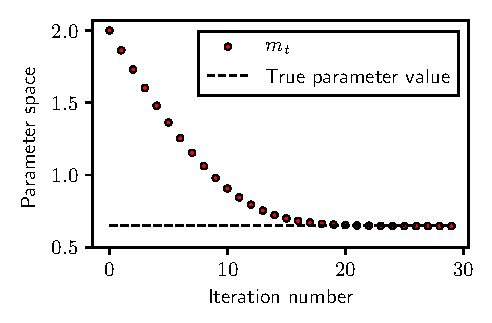
\includegraphics{figures/mm.eps}
\end{figure}

The Cram\'er-Rao Lower Bound for any unbiased estimator of $m$, say $\hat{m}$, is given as~\cite{cheng2001}
\begin{align}
    \mathrm{var}(\hat{m}) \geq \dfrac{1}{n\left(\psi'(m) - \frac{1}{m}\right)}
\end{align}

\subsection{BER in Complex $\alpha-\mu$ Fading}

Consider the system
\begin{align}
    \bm{y} = h\bm{s} + \bm{w}
\end{align}
in which $\bm{s} \in \mathbb{C}^{n\times 1}$ is a complex On-Off Keying (OOK) signal,
$h$ is a complex $\alpha-\mu$ random variable and $\bm{w}$ is a complex Gaussian process
with zero mean vector and covariance matrix equals $\sigma^2\bm{I}_n$, and $\bm{y}$ is
the received complex vector signal.

Assume that the OOK symbols are equiprobable and that there exist no interference
between the in-phase and quadrature components, then the probability of one bit error
is given as
\begin{align}
    p_{e} = \dfrac{1}{2}\left(\mathbb{P}\left(\hat{y}_i = 0 | s_{i} = 1\right)
                            + \mathbb{P}\left(\hat{y}_i = 1 | s_{i} = 0\right)\right).
\end{align}

Assume that the decoded vector $\bm{\hat{y}}$ is estimated using the minimum distance decoding
rule, i.e.,

\section{Conclusions}

\section*{Acknowledgement}
The authors would like to thank the Federal University of Campina Grande (UFCG)
and the Institute for Advanced Studies in Communications (Iecom) for supporting
this research.

\bibliographystyle{IEEEtran}
\bibliography{manuscript.bib}

\end{document}
